% Uncomment this to make slides with overlays:
%\documentclass[slides]{beamer}

% Uncomment these (but comment the above \documentclass line) to make handouts:
\documentclass[handout]{beamer}

% Uncomment these to have more than one slide per page
\usepackage{pgfpages}
\pgfpagesuselayout{2 on 1}[border shrink=5mm]
\pgfpageslogicalpageoptions{1}{border code=\pgfusepath{stroke}}
\pgfpageslogicalpageoptions{2}{border code=\pgfusepath{stroke}}

\usepackage[]{graphicx, color, hyperref}

\mode<presentation>
{
	%\usetheme[secheader]{Boadilla}
	%\usecolortheme[rgb={.835, .102,.169}]{structure}  
	\usetheme[width= 0cm]{Goettingen}
	%\setbeamercovered{transparent}
}
\setbeamertemplate{navigation symbols}{}
\setbeamertemplate{footline}[frame number]

\definecolor{blue2}{rgb}{0.278,0.278,0.729} 
\newcommand{\blue}[1]{\textcolor{blue2}{#1}}
\newcommand{\white}[1]{\textcolor{white}{#1}}
\newcommand{\red}[1]{\textcolor{red}{#1}}
\newcommand{\xbar}{\overline{x}}
\newcommand{\ybar}{\overline{y}}
\newcommand{\phat}{\widehat{p}}
\newcommand{\prob}{\mbox{Pr}}
\newcommand{\E}{\mathbb{E}}
\newcommand{\Var}{\mbox{Var}}
\newcommand{\cp}{\oplus}
\newcommand{\cm}{\circleddash}


\title{Lecture 20: Single Proportion Test}
\author{Chapter 6.1}
\date{}


\begin{document}
%------------------------------------------------------------------------------
\begin{frame}
\titlepage
\end{frame}
%------------------------------------------------------------------------------


%------------------------------------------------------------------------------
\begin{frame}[fragile]
\frametitle{Quiz 8}

\blue{Question 1}: According to the article, why do scientists even bother with correlational/observational studies, when no notions of causality can be established?

\vspace{0.5cm}

\pause\blue{Answer}:  One reason is that correlational studies are excellent starting points for deciding which hypotheses to evaluate with the more rigorous randomized controlled experiment.

\end{frame}
%------------------------------------------------------------------------------


%------------------------------------------------------------------------------
\begin{frame}[fragile]
\frametitle{Quiz 8}

\blue{Question 2}: The article argues that various scientific disciplines should set professional labeling standards for material discussed in the media...  Rank the four possible labels in order of how much creedence the public should give them, from lowest to highest.  

\vspace{0.5cm}

\pause\blue{Answer}:
\begin{enumerate}
\item[3.] preliminary result
\item[1.] large-scale observational study
\item[4.] large-sample randomized controlled test
\item[2.] well-established scientific law that we know how to apply in a wide range of conditions
\end{enumerate}

\end{frame}
%------------------------------------------------------------------------------


%------------------------------------------------------------------------------
\begin{frame}[fragile]
\frametitle{Causality}

What is causality?  How do we establish it?  

\begin{itemize}
\item \blue{\url{http://nfs.unipv.it/nfs/minf/dispense/patgen/lectures/files/disease_causality.html}}
\item \blue{\url{http://bayes.cs.ucla.edu/BOOK-2K/}}
\end{itemize}


\end{frame}
%------------------------------------------------------------------------------







%------------------------------------------------------------------------------
\begin{frame}[fragile]
\frametitle{Question for Today}

According to a (representatively sampled) poll done by the New York Times/CBS News in June 2012, only about 44\% of the American public approved of the Supreme Court's performance.  

\vspace{0.25cm}

\pause The sample proportion $\phat=0.44$ is \blue{point estimate} of $p$: the true (population) proportion of the American public who approves.  

\vspace{0.25cm}

\pause What are some next things to ask?

\vspace{0.25cm}

\pause\begin{itemize}
\item What was $n$?
\item What is the \blue{SE} of $\phat=44\%=0.44$?
\item What is the sampling distribution of $\phat$?
\end{itemize}

\end{frame}
%------------------------------------------------------------------------------


%------------------------------------------------------------------------------
\begin{frame}[fragile]
\frametitle{Question for Today}

Just like with $\xbar$, if we want to use the normal model to
\begin{itemize}
\item build confidence intervals via $z^*$
\item conduct hypothesis tests via the normal tables
\end{itemize}
we need the \blue{sampling distribution} of $\phat$ to be nearly normal.  

\vspace{0.25cm}
\pause This happens when the population distribution of 0's and 1's is not too strongly skewed.  As the sample size $n \longrightarrow \infty$, this is less of an issue by the CLT. 

%
% Comment this
%
\vspace{0.25cm}
\pause Note:  \[
\phat = \frac{x_1 + \ldots + x_n}{n} = \frac{1}{n}\sum_{i=1}^{n}x_i
\]
where each of the $x_i$'s are 0/1 success/failure \blue{Bernoulli} random variables.  
\end{frame}
%------------------------------------------------------------------------------


%------------------------------------------------------------------------------
\begin{frame}[fragile]
\frametitle{Conditions for Sampling Dist'n of $\phat$ Being Nearly Normal}
%
% Comment this
%
The sampling distribution of the \blue{sample proportion} $\phat$ based on sample size $n$ is nearly normal when

\begin{itemize}
\pause \item The observations are independent:  the 10\% rule
\pause \item We expect to see at least 10 successes and 10 failures in our sample.  This is called the \blue{success-failure condition}:
\begin{itemize}
\item $np \geq 10$
\item $n(1-p) \geq 10$ 
\end{itemize}
\end{itemize}
\end{frame}
%------------------------------------------------------------------------------


%------------------------------------------------------------------------------
\begin{frame}[fragile]
\frametitle{Conditions for Sampling Dist'n of $\phat$ Being Nearly Normal}

%
% Comment this
%
If conditions are met, then the sampling distribution of $\phat$ is nearly normal with
\begin{itemize}
\item mean $p$ (the true population proportion)
\item standard error
\[
SE_{\phat} = \sqrt{\frac{p(1-p)}{n}}
\]
\end{itemize}

\pause Note the similarity of the previous formula for the sample mean $\xbar$: 
\[
SE_{\xbar} = \frac{\sigma}{\sqrt{n}} = \sqrt{\frac{\sigma^2}{n}}
\]

\end{frame}
%------------------------------------------------------------------------------


%------------------------------------------------------------------------------
\begin{frame}[fragile]
\frametitle{What $p$ to use?}

%
% Comment this
%
But we \blue{don't know} what $p$ is.  So what $p$ do we use
\begin{itemize}
\item to check the success/failure condition?
\item for the $SE_{\phat} = \sqrt{\frac{p(1-p)}{n}}$?
\end{itemize}

\vspace{0.5cm}
For
\begin{itemize}
\pause \item Confidence intervals: plug in the \blue{point estimate} $\phat$ of p
\pause \item Hypothesis tests: plug in the \blue{null value} $p_0$ from $H_0: p=p_0$
\end{itemize}

\end{frame}
%------------------------------------------------------------------------------


%------------------------------------------------------------------------------
\begin{frame}[fragile]
\frametitle{Confidence Intervals}

Going back to the poll: $\phat=0.44$ based on $n=976$.  What is a 95\% confidence interval?

\vspace{0.25cm}

\pause Check the conditions and find SE \blue{using $p=\phat$}

\begin{itemize}
\pause \item 976 $<$ 10\% of 313 million $\Rightarrow$ independence
\pause \item Defining a success as a person approving of the job done by the Supreme Court:
\pause
\begin{itemize}
\item $976 \times \phat = 976 \times .44 = 429$ successes $\geq 10$
\item $976 \times (1-\phat) = 976 \times .56 = 547$ failures $\geq 10$
\end{itemize}
\end{itemize}
\pause
\[
SE_{\phat} = \sqrt{\frac{p(1-p)}{n}} \approx \sqrt{\frac{\phat(1-\phat)}{n}} = \sqrt{\frac{0.44(1-0.44)}{976}} = 0.016
\]
\end{frame}
%------------------------------------------------------------------------------


%------------------------------------------------------------------------------
\begin{frame}[fragile]
\frametitle{Confidence Intervals}

A 95\% confidence interval using the normal model has $z^*=1.96$, thus:
\[
\mbox{point estimate} \pm 1.96 \times SE
\]

\pause In our case
\[
\phat \pm 1.96\times SE_{\phat} = 0.44 \pm 1.96 \times 0.016 = (0.409, 0.471)
\]

\end{frame}
%------------------------------------------------------------------------------


%------------------------------------------------------------------------------
\begin{frame}[fragile]
\frametitle{Hypothesis Tests}
Thomas Carcetti is running for mayor of Baltimore.  His campaign manager \blue{claims} he has more than 50\% support of the electorate.  

\vspace{0.5cm}

\pause The Baltimore Sun collects a random sample of $n=500$ likely voters and finds that 52\% support him.  Does this provide convincing evidence for the claim of Carcetti's manager at the 5\% significance level?

\end{frame}
%------------------------------------------------------------------------------


%------------------------------------------------------------------------------
\begin{frame}[fragile]
\frametitle{Hypothesis Tests}
The hypothesis test is, with the null value $p_0=0.5$
\begin{eqnarray*}
&& H_0: p = p_0\\
\mbox{vs}&& H_A: p > p_0 
\end{eqnarray*}

\pause Check the conditions and find SE \blue{using $p=p_0$}
\begin{itemize}
\pause \item 500 $<$ 10\% of the population of Baltimore $\Rightarrow$ independence
\pause \item Success-failure condition 
\begin{itemize}
\item $np_0 = 500 \times 0.5 = 250 \geq 10$
\item $n(1-p_0) = 500 \times (1-0.5) = 250 \geq 10$
\end{itemize}
\end{itemize}
\pause
\[
SE_{\phat} = \sqrt{\frac{p(1-p)}{n}} \approx \sqrt{\frac{p_0(1-p_0)}{n}} = \sqrt{\frac{0.5(1-0.5)}{500}} = 0.022
\]

\end{frame}
%------------------------------------------------------------------------------


%------------------------------------------------------------------------------
\begin{frame}[fragile]
\frametitle{Hypothesis Tests}
\[
z = \frac{\mbox{point estimate }\phat - \mbox{ null value }p_0}{SE_{\phat}} = \frac{0.52 - 0.50}{0.022} = 0.89
\]
\pause p-value is 0.1867.  In the original \%'age scale:
\begin{center}
   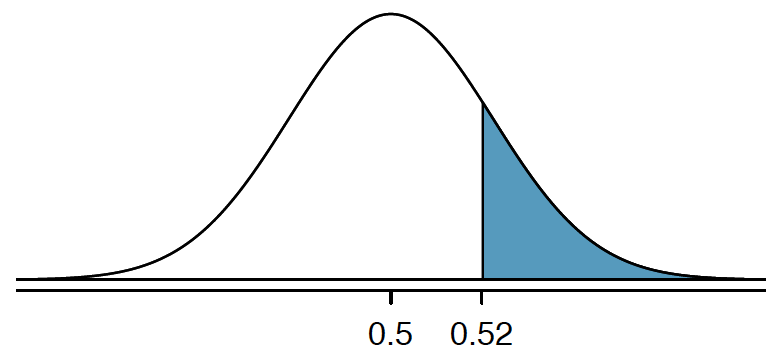
\includegraphics[width=0.6\textwidth]{figure/pvalue.png} 
\end{center}
\pause Hence we do \blue{not} reject the null hypothesis, and we do not find convincing evidence to support the campaign manager's claim.  

\end{frame}
%------------------------------------------------------------------------------


%------------------------------------------------------------------------------
\begin{frame}[fragile]
\addtocounter{framenumber}{2}
\frametitle{Next Time}

Same as with the jump from 
\[\mu \ \mbox{ to } \ \mu_1-\mu_2\] 
i.e. from one to two-sample tests for means, 
we make the jump from 
\[p \ \mbox{ to } \ p_1-p_2\]
i.e. from one to two-sample tests for proportions.
\end{frame}
%------------------------------------------------------------------------------


\end{document}


















%------------------------------------------------------------------------------
\begin{frame}[fragile]
\frametitle{Last Semester's MATH 141}
Class looked like this:
\begin{center}
   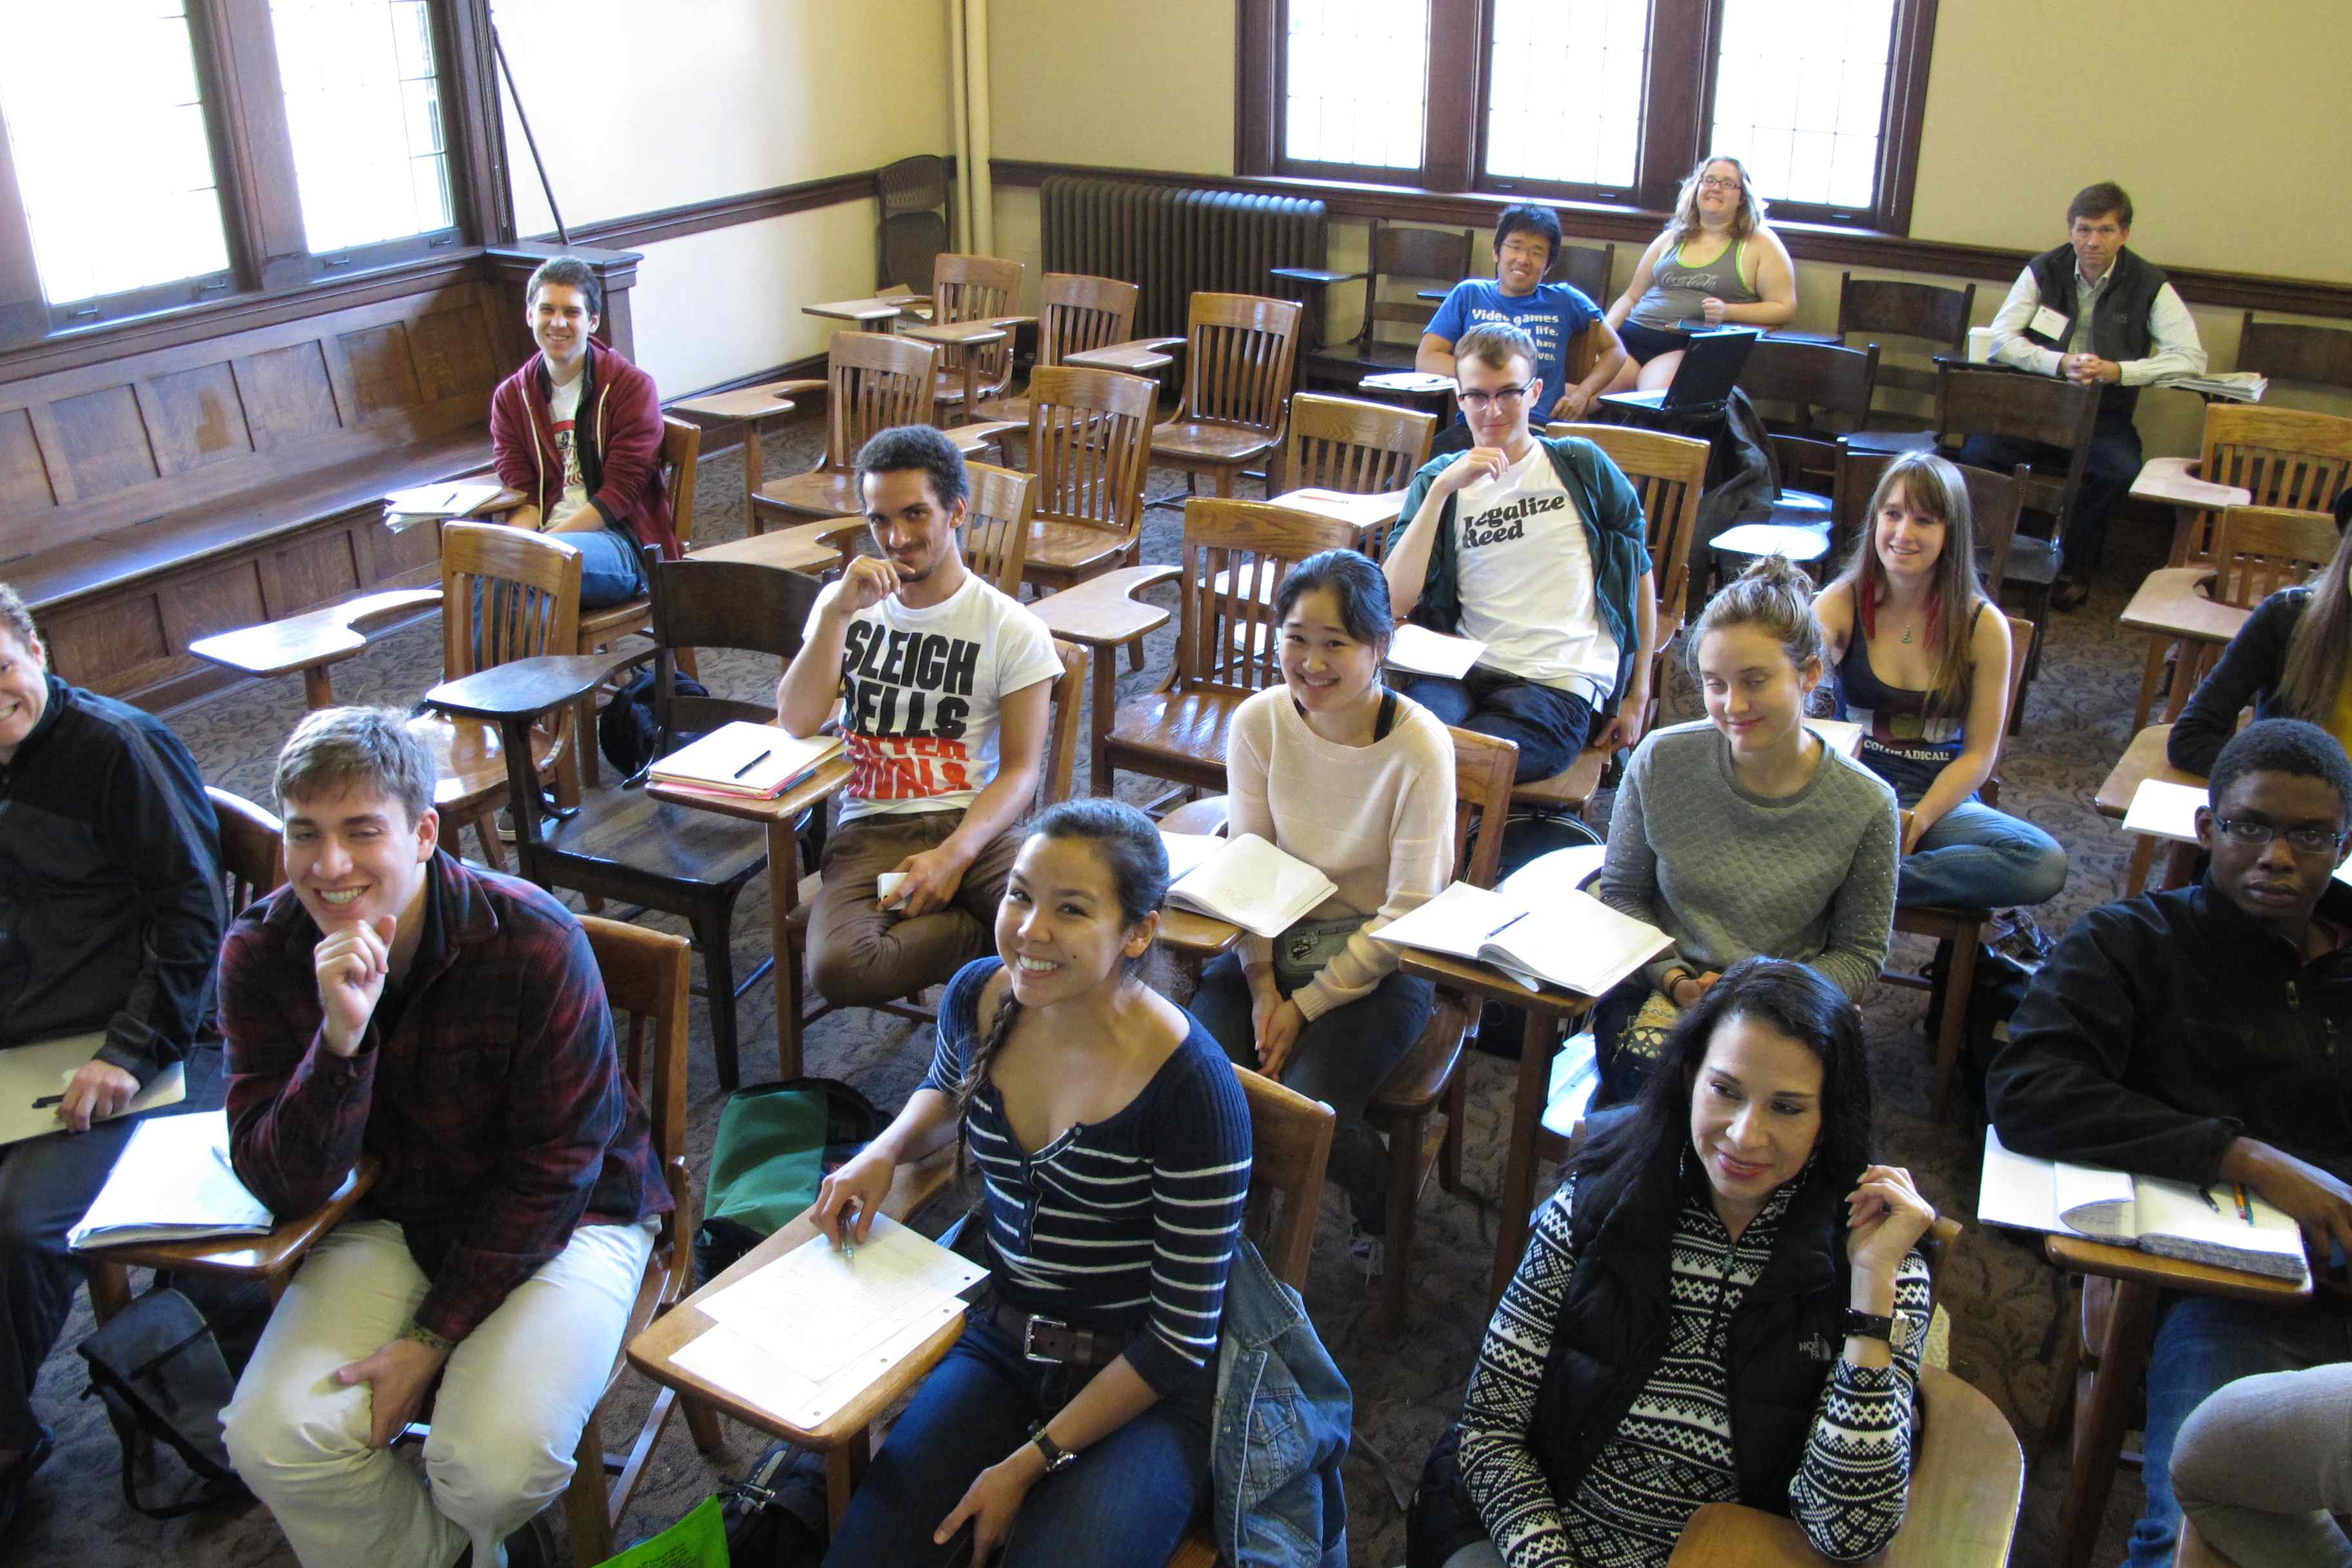
\includegraphics[width=0.5\textwidth]{Left.jpg} 
   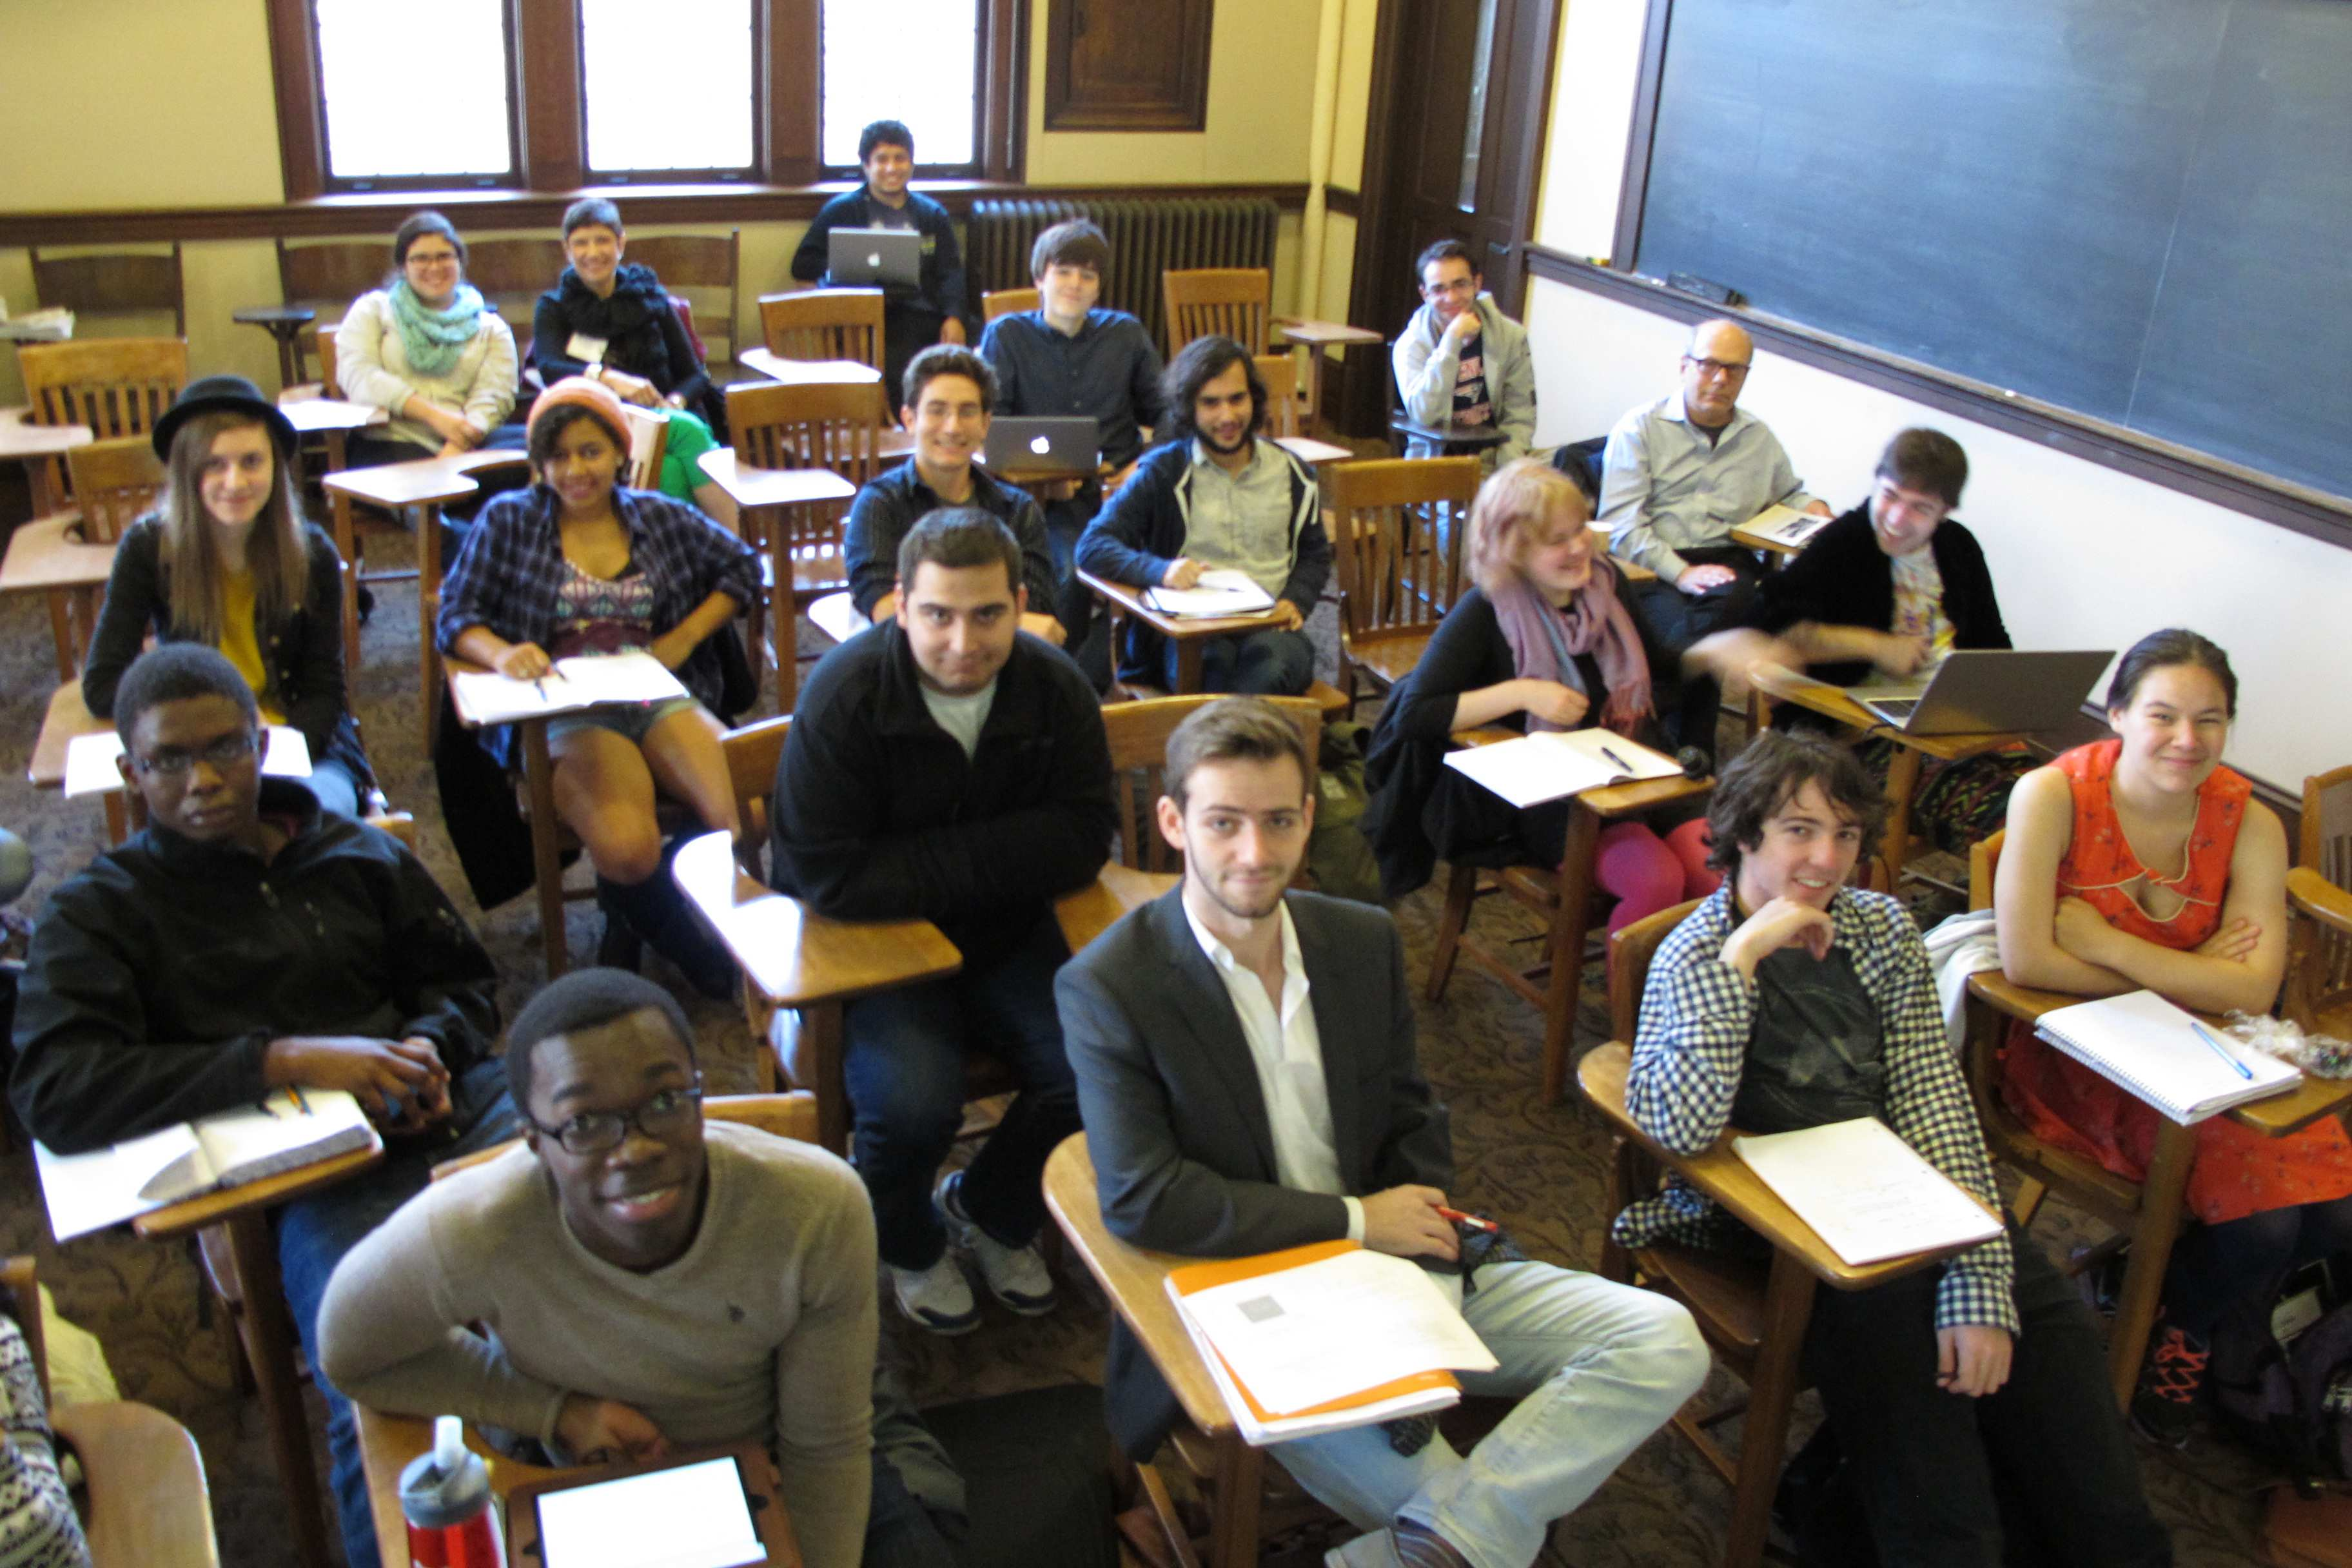
\includegraphics[width=0.5\textwidth]{Right.jpg} 
\end{center}

\end{frame}
%------------------------------------------------------------------------------


%------------------------------------------------------------------------------
\begin{frame}[fragile]
\frametitle{Questions of Interest}
I wanted to answer the following questions using data:

\begin{itemize}
\pause\item Is there a difference between the performance of students who sit to the \blue{left} of the class vs those who sit to the \blue{right}?
\pause\item Is there a difference between the performance of students who sit in the \blue{front} of the class vs those who sit in the \blue{back}?
\end{itemize}

\vspace{0.25cm}  

\pause\blue{Performance} as defined by average performance on the first 5 HW's, where each HW is weighted equally.

\end{frame}
%------------------------------------------------------------------------------



%------------------------------------------------------------------------------
\begin{frame}[fragile]
\frametitle{Seating Data}

\begin{center}
   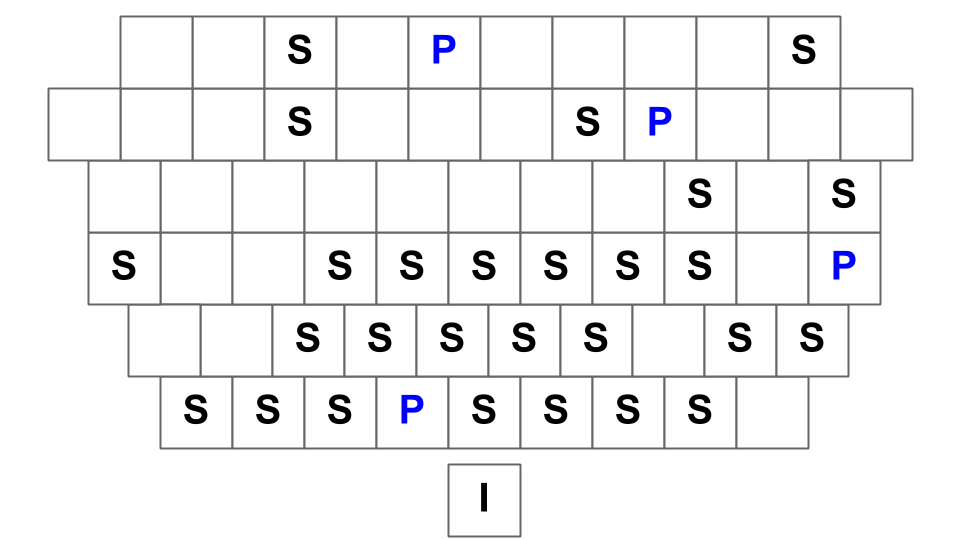
\includegraphics[width=\textwidth]{seat1.png} 
\end{center}

\end{frame}
%------------------------------------------------------------------------------


%------------------------------------------------------------------------------
\begin{frame}[fragile]
\frametitle{Absent Students}

There were four students absent on Friday.  However, I'm able to accurately guess where they sat from memory.

\vspace{0.5cm}

\pause If couldn't guess where the 4 absentees sat, their data would be missing.  This is a statistical issue with many datasets known as \blue{missing data}.  These are saved as {\tt NA}'s in {\tt R}.  

\end{frame}
%------------------------------------------------------------------------------


%------------------------------------------------------------------------------
\begin{frame}[fragile]
\frametitle{Absent Students}

\begin{center}
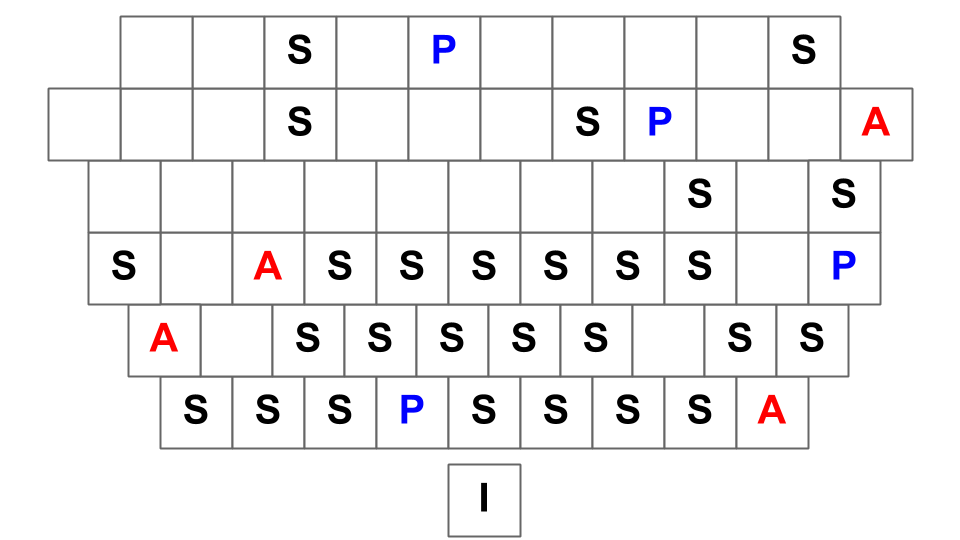
\includegraphics[width=\textwidth]{seat2.png} 
\end{center}

\end{frame}
%------------------------------------------------------------------------------


%------------------------------------------------------------------------------
\begin{frame}[fragile]
\frametitle{Drop Parents}

\begin{center}
   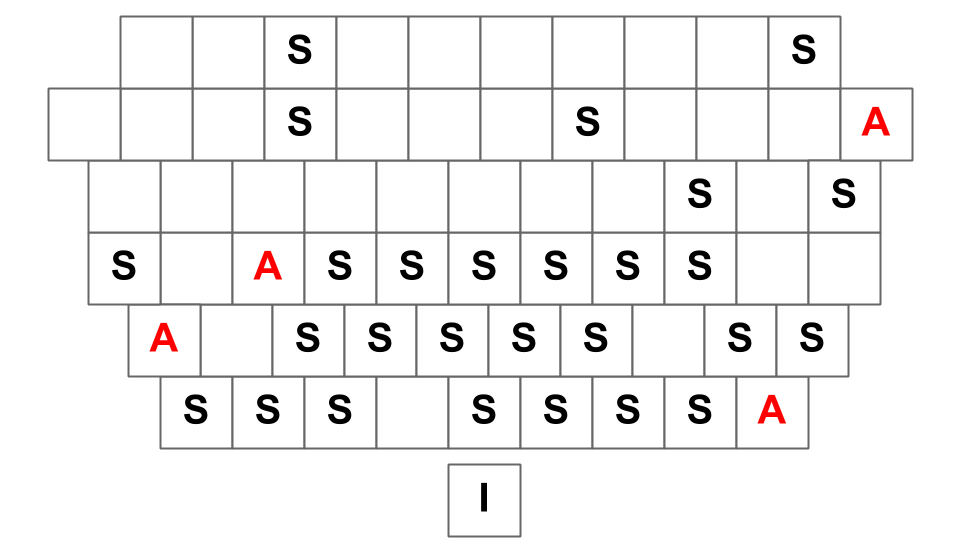
\includegraphics[width=\textwidth]{seat3.png} 
\end{center}

\end{frame}
%------------------------------------------------------------------------------


%------------------------------------------------------------------------------
\begin{frame}[fragile]
\frametitle{Forgive Absentees}

\begin{center}
   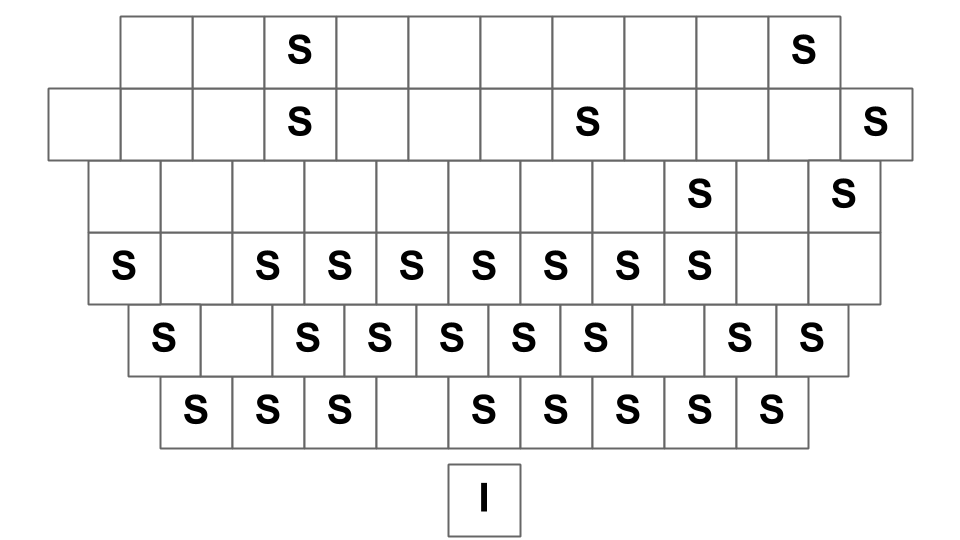
\includegraphics[width=\textwidth]{seat4.png} 
\end{center}

\end{frame}
%------------------------------------------------------------------------------


%------------------------------------------------------------------------------
\begin{frame}[fragile]
\frametitle{Division of Classroom}

We now divide the classroom into quadrants that define
\begin{itemize}
\item Front/Back:  6 rows of seats, so let's take front 3 rows, and back 3 rows
\item Left/Right:  Split down the middle
\end{itemize}

\end{frame}
%------------------------------------------------------------------------------


%------------------------------------------------------------------------------
\begin{frame}[fragile]
\frametitle{Potential Division of Classroom}
\begin{center}
   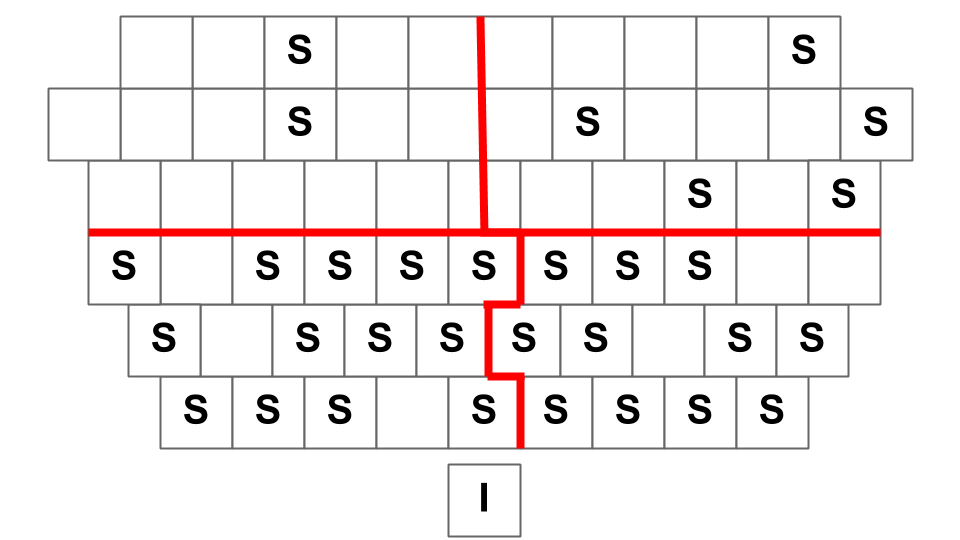
\includegraphics[width=\textwidth]{seat5.png} 
\end{center}

\end{frame}
%------------------------------------------------------------------------------


%------------------------------------------------------------------------------
\begin{frame}[fragile]
\frametitle{Issue with Potential Division of Classroom}

\begin{itemize}
\pause\item Only 2 people in the Back-Left quadrant.  Not an issue per se.  We can still conduct statistical tests, although more balance might be better.
\pause\item \blue{Confidentiality!}  A more practical consideration:  If we show a histogram of these two scores, we can almost identify who got what!
\end{itemize}

\end{frame}
%------------------------------------------------------------------------------


%------------------------------------------------------------------------------
\begin{frame}[fragile]
\frametitle{Proposed Division of Classroom}

\begin{center}
   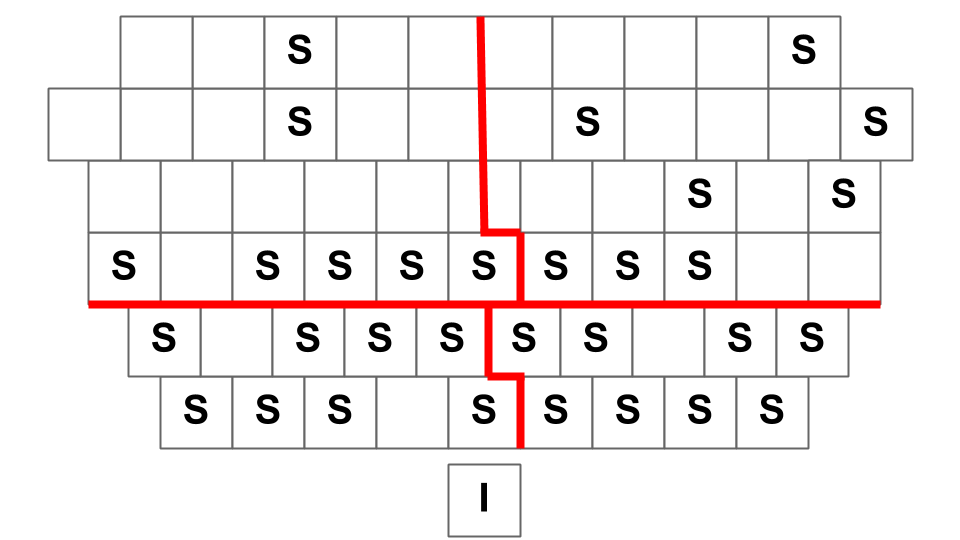
\includegraphics[width=\textwidth]{seat6.png} 
\end{center}

\end{frame}
%------------------------------------------------------------------------------


%------------------------------------------------------------------------------
\begin{frame}[fragile]
\frametitle{Balanced Sample Sizes}

\begin{center}
   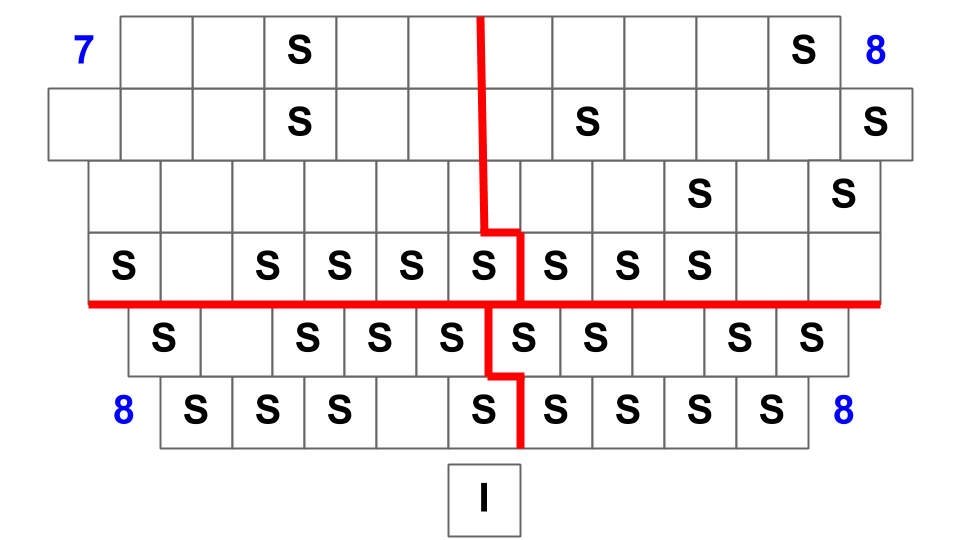
\includegraphics[width=\textwidth]{seat7.png} 
\end{center}

\end{frame}
%------------------------------------------------------------------------------


%------------------------------------------------------------------------------
\begin{frame}[fragile]
\frametitle{Balanced Sample Sizes}

\begin{center}
   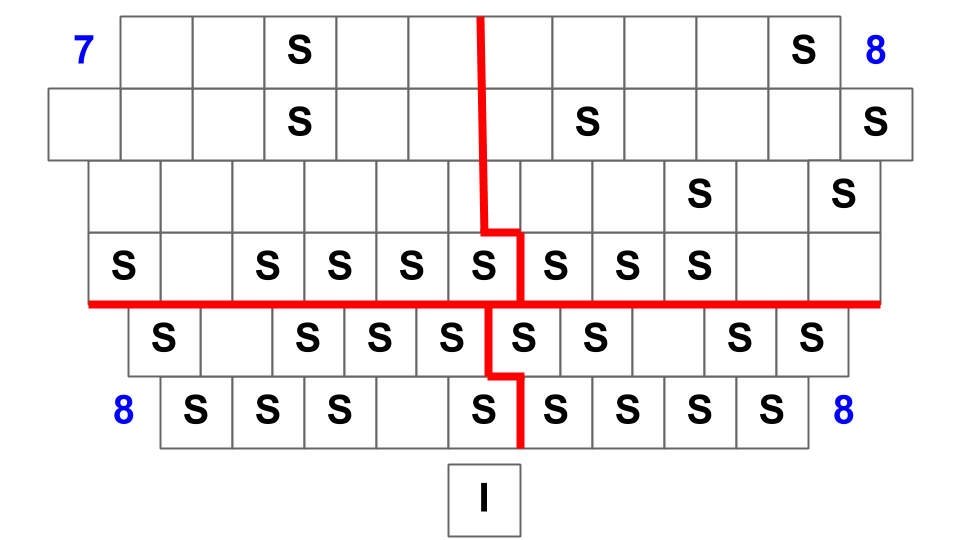
\includegraphics[width=\textwidth]{seat7.png} 
\end{center}

\end{frame}
%------------------------------------------------------------------------------


%------------------------------------------------------------------------------
\begin{frame}[fragile]
\frametitle{Results}

And the results...

\pause will be investigated by you in lab on Tuesday.  

\end{frame}
%------------------------------------------------------------------------------










